\documentclass[11pt,a4paper]{jarticle}
\usepackage[dvipdfmx]{graphicx}
\usepackage{url}

\renewcommand{\baselinestretch}{1.05} 
\marginparwidth=0cm
\topmargin=-1cm
\headheight=0.3cm
\headsep=0.7cm
\oddsidemargin=0cm
\evensidemargin=0cm
%\textwidth=43zw
\textwidth=15.92cm
%\textheight=43.3\baselineskip
\baselineskip = 0.5744cm
\textheight=43\baselineskip

\itemsep=0.05\baselineskip
\parsep=0pt
\topsep=0.01\baselineskip
\partopsep=0pt
\listparindent=0zw

%% header and footer
\usepackage{fancyhdr}
\pagestyle{fancy}
\lhead{2014年度 春学期授業}
\chead{インタラクティブ・アート実習}
\rhead{担当教員: 松下 光範}
\cfoot{\thepage}
\renewcommand{\headrulewidth}{0pt}
\renewcommand{\footrulewidth}{0pt}

\usepackage{ascmac}
\usepackage{listings,jlisting}
\usepackage{color}
\definecolor{OliveGreen}{cmyk}{0.64,0,0.95,0.40}
\definecolor{colFunc}{rgb}{1,0.07,0.54}
\definecolor{CadetBlue}{cmyk}{0.62,0.57,0.23,0}
\definecolor{Brown}{cmyk}{0,0.81,1,0.60}
\definecolor{colID}{rgb}{0.63,0.44,0}
\definecolor{rulesepcolor}{gray}{0.666}
\lstset{
  language=Java,%プログラミング言語によって変える。
  basicstyle={\ttfamily\small},
  keywordstyle={\color{OliveGreen}},
  %[2][3]はプログラミング言語によってあったり、なかったり
  keywordstyle={[2]\color{colFunc}},
  keywordstyle={[3]\color{CadetBlue}},%
  commentstyle={\color{Brown}},
  %identifierstyle={\color{colID}},
  stringstyle=\color{blue},
  tabsize=2,
  %frame=trBL,
  %numbers=left,
  numberstyle={\ttfamily\small},
  breaklines=true,%折り返し
  %backgroundcolor={\color[gray]{.95}},
  framexleftmargin=0mm,
  frame=single,
  rulesepcolor=\color{rulesepcolor},
  captionpos=b
}


%%%%%%%%%%%%%%%%%%%%%%%%%%%%%%%%%%%%%%%%%%%%%%%%%%%%%%%%%%%%%%%%
\begin{document}
% title
\section*{\LARGE{第5講 様々なセンサを用いる}}
Arduino の Analog Input を用いて光センサや圧力センサの値を取得してみよう。

%%%%%%%%%%%%%%%%%%%%%%%%%%%%%%%%%%%%%%%%%%%%%%%%%%%%%%%%%%%%%%%%

\section{Processingの画面に文字を表示する}
Processing では、矩形や円のような図形だけではなく、文字を描くこともできます。
文字を表示するには text() を用います。
また、 PFont と textFont() を用いることによってフォントの種類や大きさを変更することができます。

PFont を用いて任意のフォントを使用するためには、フォントファイルを用意しなければなりませんが、
Processing には簡単にフォントファイルを用意するための機能が備わっています。
\begin{enumerate}
 \item メニューから Tools → Create Font を選択する
 \item 使いたいフォントを選択する
 \item フォントの名前が表示されているのを確認する (例、Serif-48.vlw ← コイツを覚えておくこと!)
 \item OK ボタンを押す
\end{enumerate}
これで、data フォルダ\footnote{作成しているプログラムと同じフォルダの中にある。フォントファイルや画像ファイルなど、プログラムから読み込みたいファイルなどはここに入れておくとよい。メニューの Sketch → Show Sketch Folder から作成しているプログラムが入っているフォルダを開ける。}
の中にフォントファイルが生成されたと思います。
loadFont() を用いて生成したフォントファイルを読み込むことで、好きなフォントを使うことができます

% 分かり難いので図を入れる!
% めんどい

\begin{lstlisting}
 PFont font;

 void setup() {
   size(300, 300);

   // Create Font で作ったフォントを読み込む
   font = loadFont("Serif-48.vlw");
 }

 void draw() {
   background(255);

   textFont(font, 32); // 使うフォントとその大きさの指定
   fill(0);
   text("Interactive Art", 64, 64); // 文字を描く
 }
\end{lstlisting}
ウィンドウの中に Interactive Art の文字列が表示されると思います。
できましたか?

\newpage

\section{Analog Input}
Arduino には、Analog Output と同様に Analog Input もあります。
Analog Input を用いる場合は A0 〜 A5 ピンに接続してください。

Processing から Analog Input を使って値を取得するには、
\begin{lstlisting}
 arduino.analogRead(pinNum);
\end{lstlisting}
を用います。
pinNum は 0 〜 5 (それぞれ、A0 〜 A5 に対応) で指定してください。
Digital Input を用いたときのような、PINモードの設定は必要ありません。

\begin{figure}[h!]
 \centering
 \includegraphics[width=0.6\columnwidth]{img/analog_input_pins.eps}
\end{figure}

\section{光センサを使う}
光センサとは、表面に当たる光の量に従って抵抗値が変化する電子部品です。
周りが暗いと抵抗値が大きくなり、明るいと抵抗値が小さくなります。
テスターを使って抵抗値の変化を測ってみましょう。

実習で使う光センサは CdSセル (CdS: 硫酸カドミウム) を主成分とするものです。

\begin{figure}[h!]
 \begin{minipage}{0.666\columnwidth}
  \begin{itemize}
   \item \textbf{利点}
	 \begin{itemize}
	  \item 可視光線に対して高感度
	  \item 小型で軽量
	  \item 比較的安価
	 \end{itemize}
   \item \textbf{欠点}
	 \begin{itemize}
	  \item 反応速度がやや遅め
	  \item カドミウム = 有害物質 (ゼッタイに食うな!)
	 \end{itemize}
  \end{itemize}
 \end{minipage}
 \begin{minipage}{0.333\columnwidth}
  \centering
  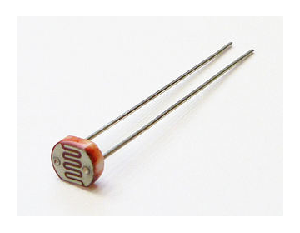
\includegraphics[width=\columnwidth]{img/cds_cell.eps}
  \caption{CdS セル}
 \end{minipage}
\end{figure}


\subsection*{光センサの値を取得する}
光センサの値を取得するためには、Analog Input を用います。
Analog Input を使う場合は前述のように A0 〜 A5 ピンを用いる必要があります。
接続するピンに注意してください。

\subsubsection*{回路}
\begin{figure}[h!]
 \centering
 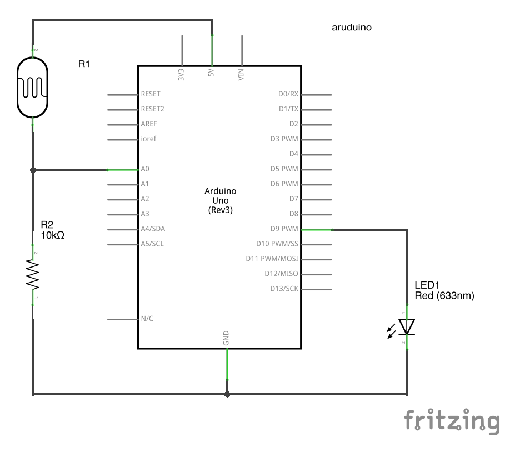
\includegraphics[width=0.5\columnwidth]{img/light_sensor.eps}
 \caption{光センサの回路図}
\end{figure}


\subsubsection*{プログラム}
\begin{lstlisting}
 import processing.serial.*;
 import cc.arduino.*;
 
 Arduino arduino;
 int sensorPin = 3; // 光センサを A3 番ピンに接続した場合
 PFont font;
 
 void setup() {
   size(300, 300);

   arduino = new Arduino(this, Arduino.list()[0]);
   font = loadFont("Serif-48.vlw");
 }

 void draw() {
   background(255);

   int sensorValue = arduino.analogRead(sensorPin); // Analog Input

   textFont(font, 32);
   fill(0);
   text("sensor value: " + sensorValue, 64, 64);
 }
\end{lstlisting}

\newpage

\section{圧力センサを使う}
圧力センサとは、感圧面に加重することにより抵抗値が変化するセンサです。
タクトスイッチなどの、ON/OFF を検出するスイッチとは違い、押した強さを検出できます。

回路とプログラムは光センサのときと同様です。
光センサを圧力センサに差し替えれば使えます。
やってみましょう。

圧力センサ (や曲げセンサなど) は、LED や抵抗、光りセンサなどの部品よりも\textbf{非常に高価なので壊さないように注意してください!}
\begin{itemize}
 \item ピンが折れやすいので注意すること!
 \item ブレッドボードに差すときは、ピンに近い部分を持つこと (無理に差さないように)
 \item フィルム部分を曲げすぎないように
\end{itemize}


\section{曲げセンサを使う}
曲げセンサとは、センサ本体を曲げることにより抵抗値が変化するセンサです。
プリント面を外側にした状態で曲げると抵抗値が増加します。
1つの曲げセンサだけでは、片方向への曲げしか検出できませんが、2つを重ねて用いることによって、両方向の曲げを検出できます。

曲げセンサも光センサや圧力センサと同様に使えます。
すみませんが今回は前で見せるだけにします。
% 前で見せますが高いのでおまえらにはやらねー。←糞ワロリッシュタイフーン

\begin{figure}[h!]
 \begin{minipage}{0.5\columnwidth}
  \centering
  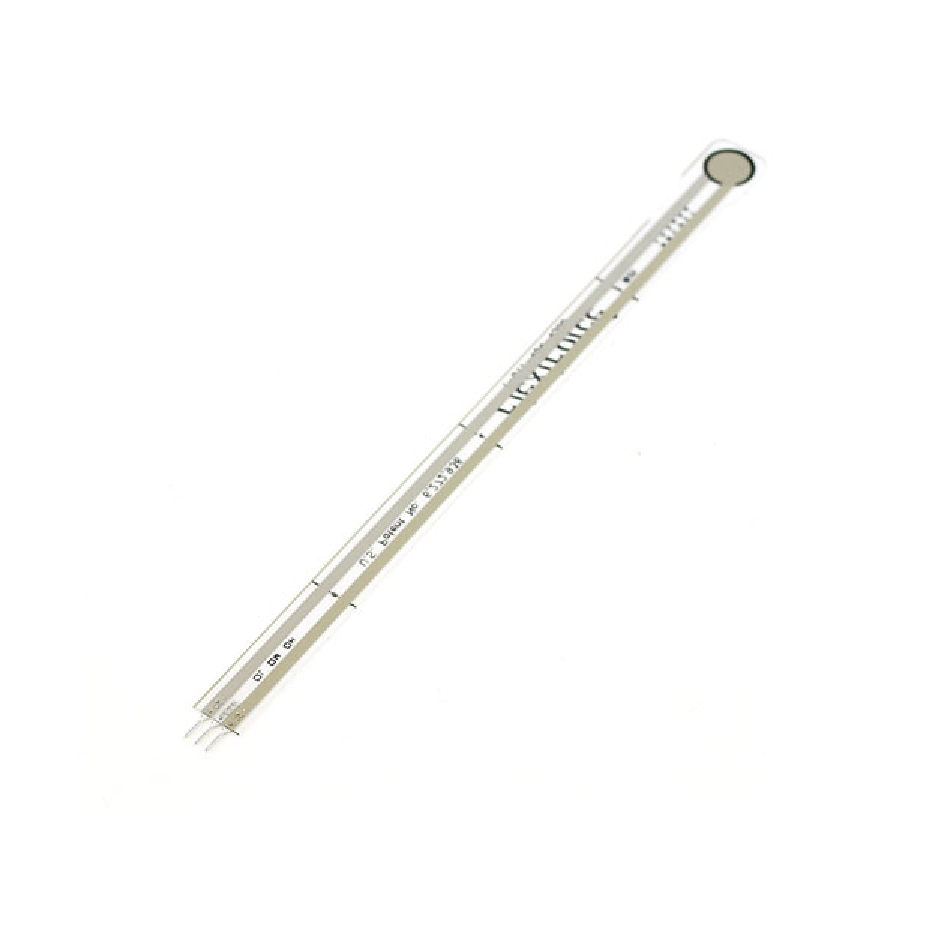
\includegraphics[width=\columnwidth]{img/pressure_sensor.eps}
  \caption{圧力センサ}
 \end{minipage}
 \begin{minipage}{0.5\columnwidth}
  \centering
  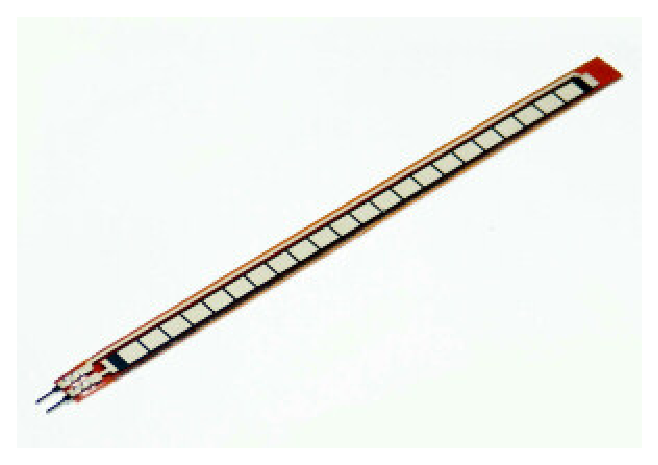
\includegraphics[width=\columnwidth]{img/flex_sensor.eps}
  \caption{曲げセンサ}
 \end{minipage}
\end{figure}
\end{document}